\documentclass[tikz, margin=3mm]{standalone}
\usetikzlibrary{arrows.meta, bending, calc, chains,  positioning, shapes}

\begin{document}
    %\begin{figure}[!h]  % when use article \documentclass{article}
    %\centering          % when use article \documentclass{article}
    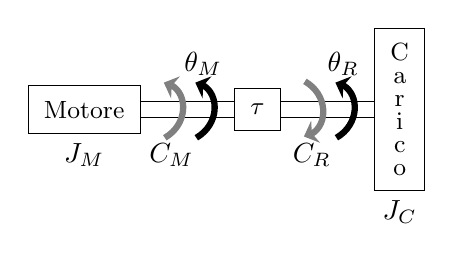
\begin{tikzpicture}[
node distance = 0mm,
  start chain = going right,
   box/.style = {draw,
                 font=\linespread{0.75}\selectfont\small,
                 align=center, inner sep=2mm, outer sep=0pt,
                 on chain},
   axs/.style = {draw, minimum width=12mm, minimum height=2mm,
                 inner sep=0pt, outer sep=0pt,
                 on chain, node contents={}},
   arr/.style = {color=#1, line width=0.8mm, 
                 shorten >=-1mm, shorten <=-1mm,
                 -{Stealth[length=1.6mm,width=3mm,flex=1.2]},
                 bend angle=60}
                        ]
    % blocks (boxes)
\node (n1) [box,label=below:$J_M$]  {Motore};
\node (n2) [axs];
\node (n3) [box]                    {$\tau$};
\node (n4) [axs];
\node (n5) [box,label=below:$J_C$]  {C\\a\\r\\i\\c\\o};
    % arrows
\draw[transform canvas={xshift=-2mm}]
    (n1.south -| n2) edge[arr=gray,bend right] (n1.north -| n2)
                     node[below,at={(n1.south -| n2)}] {$C_M$}                     
    (n1.north -| n4) edge[arr=gray,bend  left] (n1.south -| n4)
                     node[below,at={(n1.south -| n4)}] {$C_R$};
\draw[transform canvas={xshift=+2mm}]
    (n1.south -| n2) edge[arr=black,bend right] (n1.north -| n2)
                     node[above,at={(n1.north -| n2)}] {$\theta_M$}
    (n1.south -| n4) edge[arr=black,bend right] (n1.north -| n4)
                     node[above,at={(n1.north -| n4)}] {$\theta_R$};
\end{tikzpicture}
    %\end{figure} % when use article \documentclass{article}
\end{document}